\section{\normalsize Эффект Джоуля--Томсона (дифференциальный и интегральный). Температура инверсии.} 
\paragraph{Дифференциальный эффект Джоуля--Томпсона.} Рассмотрим процесс Джоуля--Томпсона: адиабатическое стационарное течение газа через пористую перегородку, под действием разности давлений

\begin{wrapfigure}{L}{7cm}
	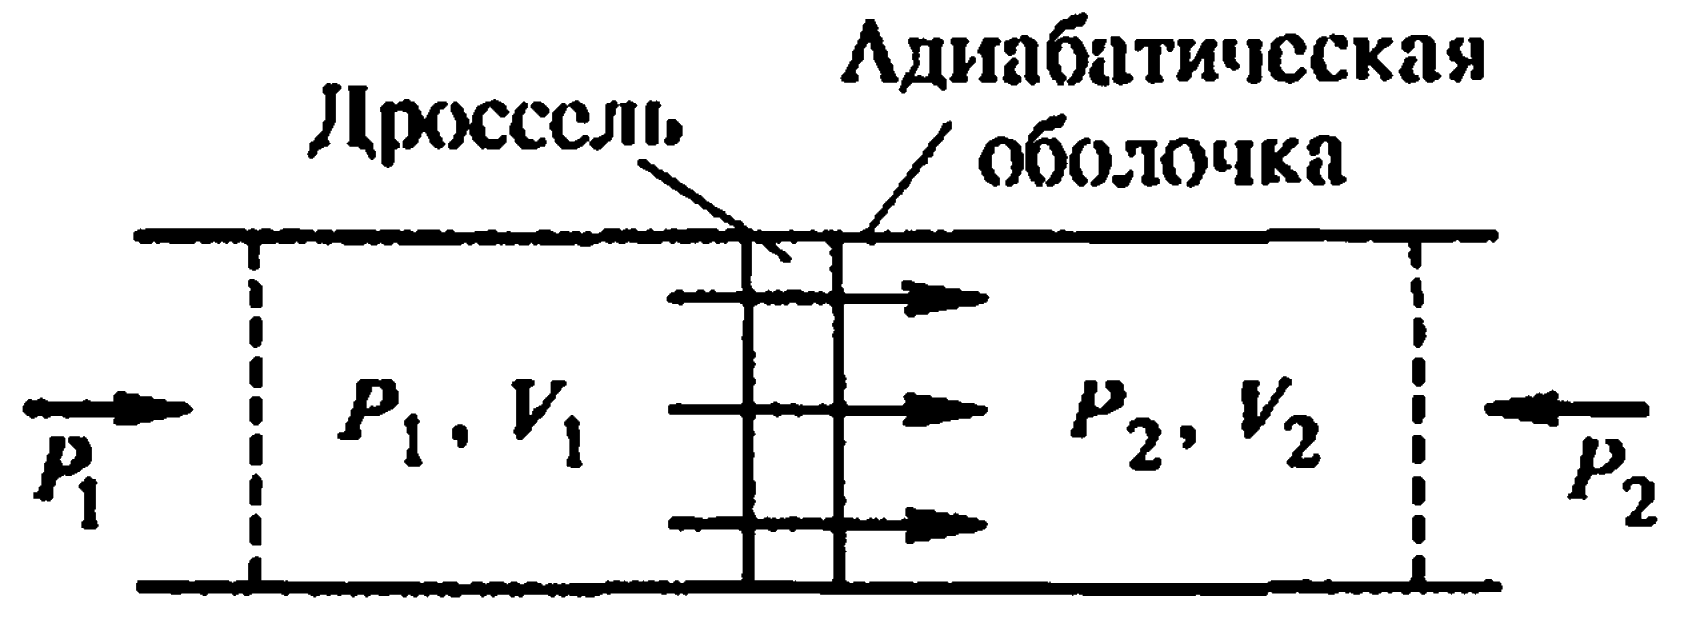
\includegraphics[width=70mm]{ris22_1.png}
\end{wrapfigure}
 по разные стороны от пробки. Изменение температуры в этом процессе --- \textbf{эффект Джоуля-Томпсона}. Течение медленное, следовательно можно пренебречь кинетической энергией. Тогда по первому началу термодинамики $Q=0\Rightarrow\\0=\Delta U+A=U_2-U_1+P_2V_2-P_1V_1=I_2-I_1\Leftrightarrow I_1=I_2$. В процессе Джоуля--Томпсона $I=const$.\\
 Пусть теперь по разные стороны от перегородки разность давлений мала. Найдем $\Delta T:$ $$\Delta I = \chpr{I}{T}{P}\Delta T+\chpr{I}{P}{T}\Delta P=0\Rightarrow\chpr{I}{T}{P}=C_P,\ \chpr{I}{P}{T}=V-T\chpr{V}{T}{P}\Rightarrow$$
 $$\Rightarrow\left(\dfrac{\Delta T}{\Delta P}\right)_I=\dfrac{T\Chpr{V}{T}{P}-V}{C_P}$$
 Если газ идеальный, то $V=\dfrac{RT}{P},\ T\chpr{V}{T}{P}=V\Rightarrow\Delta T=0$, то есть для идеальных газов эффекто Джоуля--Томпсона не имеет места. Повышение или понижение температуры реального газа при протекании через пробку при малых $\Delta T$ и $\Delta P$ $\left(\text{для замены их отношения на } \Chpr{T}{P}{I}\right)$ называется \textbf{дифференциальным эффектом Джоуля--Томпсона}.\\
 Так как течение происходит от большего давления к меньшему, то $\Delta P<0$, значит если $\frac{\Delta T}{\Delta P}>0$, то эффекто Джоуля--Томпсона \textbf{положительный}, а если соответственно $\frac{\Delta T}{\Delta P}<0$ --- \textbf{отрицательный}.
 
 \begin{wrapfigure}{R}{4cm}
 	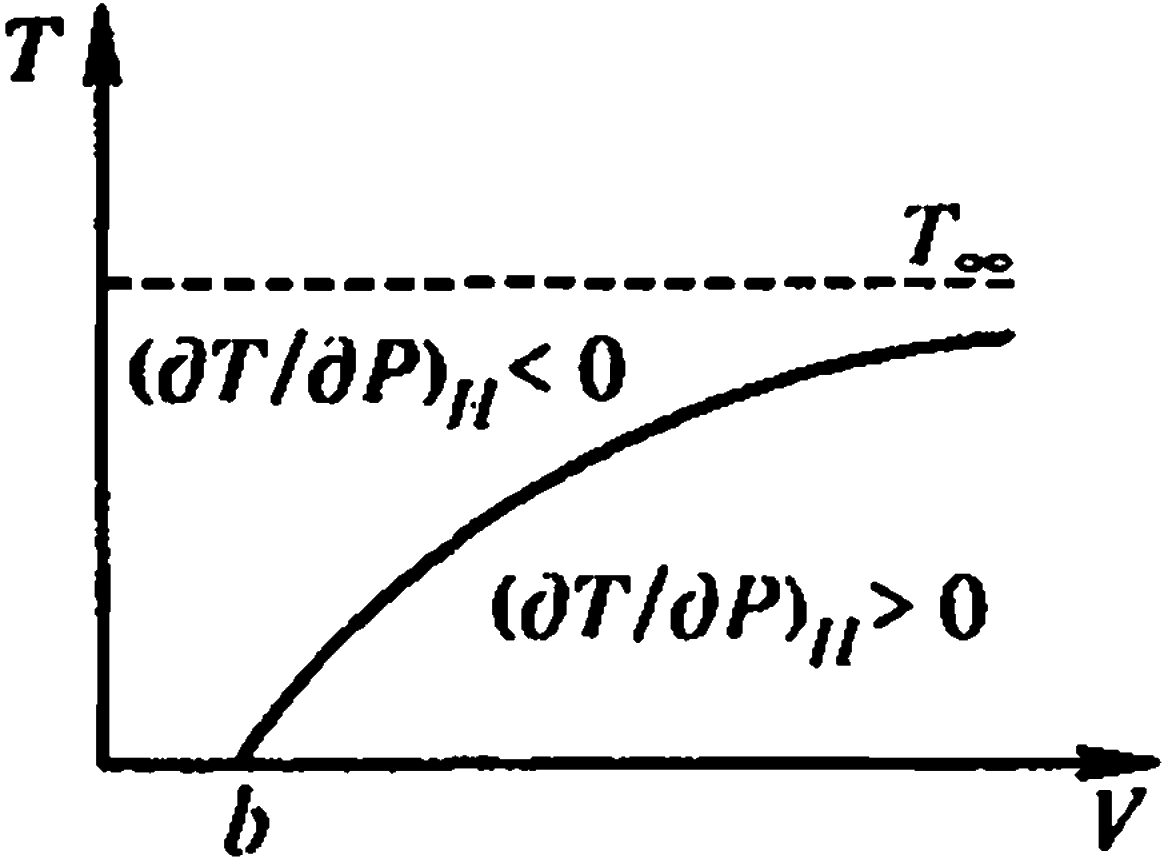
\includegraphics[width=40mm]{ris22_2.png}
 \end{wrapfigure}
 Вычисляя $\chpr{V}{T}{P}=\dfrac{-\Chpr{P}{T}{V}}{\Chpr{P}{V}{T}}$ из уравнения Ван-дер-Ваальса получаем:
 $$\dfrac{\Delta T}{\Delta P}=-\dfrac{T\Chpr{P}{T}{V}+V\Chpr{P}{V}{T}}{C_P\Chpr{P}{V}{T}}=\dfrac{\frac{bRT}{(V-b)^2}-\frac{2a}{V^2}}{C_P\Chpr{P}{V}{T}}$$
 \paragraph{Температура инверсии.} Пояснение к графику: $T_\infty\equiv T_i,\ H\equiv I$. В случае разреженного газа можно отбросить малые поправки $a$ и $b$ высших порядков $\Rightarrow\dfrac{\Delta T}{\Delta P}=\dfrac{\frac{2a}{RT}-b}{C_P}$. При $T_i=\dfrac{2a}{RB}=\dfrac{27}{4}T_\text{кр.}$ --- температуре инверсии дифференциального эффекта Джоуля--Томпсона  $\Delta T=0$. Газ ниже этой температуры охлаждается, выше --- нагревается в процессе Джоуля--Томпсона. \\
 \paragraph{Интегральный эффект Джоуля--Томпсона.} Пусть теперь по разные стороны от перегородки $\Delta P$ велика, тогда велика и $\Delta T$. 